%% Overleaf			
%% Software Manual and Technical Document Template	
%% 									
%% This provides an example of a software manual created in Overleaf.

\documentclass{../ol-softwaremanual}

% Packages used in this example
\usepackage{graphicx}  % for including images
\usepackage{microtype} % for typographical enhancements
\usepackage{minted}    % for code listings
\usepackage{amsmath}   % for equations and mathematics
\setminted{style=friendly,fontsize=\small}
\renewcommand{\listoflistingscaption}{List of Code Listings}
\usepackage{hyperref}  % for hyperlinks
\usepackage[a4paper,top=4.2cm,bottom=4.2cm,left=3.5cm,right=3.5cm]{geometry} % for setting page size and margins

\usepackage[english, greek]{babel}

\usepackage{subfig}




% Custom macros used in this example document
\newcommand{\doclink}[2]{\href{#1}{#2}\footnote{\url{#1}}}
\newcommand{\cs}[1]{\texttt{\textbackslash #1}}

\begin{document}
	
	
	\begin{titlepage}
		
		
		% Frontmatter data; appears on title page
		\title{\en Class Diagram \\}
		\version{1.0}
		\softwarelogo{
\includegraphics[scale=0.4]{../CarBazaar_logo.png}}
	\end{titlepage}
	
	
	\maketitle
	
	\newpage
	
	\center{\textbf{Μέλη Ομάδας}}
	
	\vspace{20pt}
	
	
	
	\begin{table}[htbp!]
		
		\begin{tabular}{llll}
			Μεμελετζόγλου Χαρίλαος & 1069364 & \en st1069364@ceid.upatras.gr & 4o Έτος   \\ 
			\\ Λέκκας Γεώργιος      &      1067430    &   \en st1067430@ceid.upatras.gr & 4o Έτος  \\
			\\ Γιαννουλάκης Ανδρέας        &   1067387       & \en st1067387@ceid.upatras.gr & 4o Έτος           \\
			\\ Κανελλόπουλος Ιωακείμ        &  1070914        &    \en st1070914@ceid.upatras.gr & 4o Έτος        \\ 
		\end{tabular}
	\end{table}
	
	\center{\textbf{Υπεύθυνοι Παρόντος Τεχνικού Κειμένου}}
	
	\vspace{20pt}
	
	\begin{table}[htbp!]
		\begin{tabular}{ll}
			Μεμελετζόγλου Χαρίλαος & \en Editor \\
			\\ Λέκκας Γεώργιος      &   \en  Editor \\
			\\ Γιαννουλάκης Ανδρέας & \en Peer Reviewer \\
			\\ Κανελλόπουλος Ιωακείμ & \en Peer Reviewer \\ 
		\end{tabular}
	\end{table}
	
	\center{\textbf{Αλλαγές στην έκδοση \en v1.0\gr}}
	\flushleft
	
	Μετονομασία της μεθόδου \en \textbf{add\_part\_to\_category()} \gr της κλάσης \en \textit{SparePart} \gr, σε \en \textbf{add\_spare\_part\_to\_category()} \gr. \break
	
	Προσθήκη της μεθόδου \en \textbf{get\_photos()} \gr στην κλάση \en \textit{Listing} \gr. \break
	
	Προσθήκη της μεθόδου \en\textbf{get\_car\_condition()} \gr στην κλάση \en\textit{CarListing}\gr. \break
	
	Τροποποίηση της μεθόδου \en\textbf{check\_location\_validity()} \gr της κλάσης \en \textit{Location}\gr. Συγκεκριμένα, η μέθοδος πλέον δεν έχει ορίσματα. \break
	
	Αλλαγή της σειράς των ορισμάτων της μεθόδου \en\textbf{set\_ad\_info()} \gr της κλάσης \en\textit{Advertisement}\gr. \break
	

	
	Αλλαγή των ορισμάτων της μεθόδου \en\textbf{set\_car\_inspection\_info()} \gr της κλάσης \en \textit{CarInspection} \gr. Επίσης, στην ίδια κλάση προστέθηκαν οι μέθοδοι \en\textbf{set\_car\_inspection\_transaction(), set\_car\_to\_inspect(), start\_car\_inspection(), finish\_car\_inspection()}\gr. Ακόμη, η μέθοδος \en \textbf{find\_inspector()} \gr, μετονομάστηκε σε \en \textbf{find\_recommended\_inspector()} \gr, και το \en return type \gr της άλλαξε, από \en List [ ] \gr, σε \en User \gr. 
	
	Ακόμη, άλλαξε το \en return type \gr της μεθόδου \en\textbf{\textit{set\_car\_inspection\_inspector()}} \gr από \en bool \gr σε \en void \gr και προστέθηκε η μέθοδος \en \textbf{\textit{find\_inspector()}} \gr, η οποία δέχεται ως ορίσματα το τηλέφωνο και το \en email \gr ενός Ελεγκτή, ελέγχει αν υπάρχει εγγεγραμμένος Ελεγκτής με αυτά τα στοιχεία επικοινωνίας και επιστρέφει το \en instance \gr του Ελεγκτή αυτού.
	
	Τέλος, στην ίδια κλάση, προστέθηκε η μέθοδος \en\textbf{get\_inspector()}\gr. \break
	
	Προσθήκη των μεθόδων \en\textbf{start\_car\_transportation(), finish\_car\_transportation()} \gr στην κλάση \en \textit{CarTransportation}\gr. Επίσης, στην ίδια κλάση έγινε μετονομασία της μεθόδου \en\textbf{set\_transportation\_info()} \gr σε \en\textbf{set\_car\_transportation\_info()} \gr. \break
		
	
	Προσθήκη του πεδίου \en \textbf{\textit{reviews}} \gr, τύπου \en Review [ ] \gr, στην κλάση \en \textit{User} \gr, το οποίο περιέχει τις κριτικές που έχει δεχθεί ένας χρήστης. Προσθήκη των μεθόδων \en\textbf{add\_user\_review(), get\_reviews\_list()} \gr, στην ίδια κλάση. \break
	
	
	Αφαίρεση του ορίσματος τύπου \en Date \gr από την μέθοδο \en \textbf{set\_review\_info()} \gr της κλάσης \en \textit{Review}\gr. Επίσης, στην ίδια κλάση προστέθηκε η μέθοδος \en \textbf{is\_review\_positive()} \gr, που επιστρέφει \en True \gr, αν μια κριτική είναι θετική (θεωρούμε πως \textit{θετικές} είναι οι κριτικές που έχουν πάνω από \textit{3} αστέρια). \break
	
	Αφαιρέθηκε η κλάση \en \textbf{Photograph} \gr, καθώς στην υλοποίηση η εν λόγω κλάση, κρίθηκε μη-απαραίτητη μιας και χρησιμοποιήθηκε η κλάση \en \textit{QPixmap} \gr, του \en PyQt framework \gr. \break
	
	Τέλος, σε αρκετές κλάσεις έγινε αναδιάταξη της σειράς αναγραφής των μεθόδων, ώστε αυτή να συμπίπτει με την σειρά εμφάνισής τους στο αρχείο του κώδικα (\en \textit{classes.py}\gr). 
	

	
	
	\center{\textbf{Εργαλεία που χρησιμοποιήθηκαν}}
	

	\flushleft
	Χρησιμοποιήθηκε το \en \doclink{https://www.overleaf.com/}{Overleaf} \gr και το \en \doclink{https://www.texstudio.org/}{TexStudio} \gr για την συγγραφή του \LaTeX\ κώδικα. \break
	
	Για την δημιουργία του \en Class Diagram \gr χρησιμοποιήθηκε το \en \doclink{https://www.visual-paradigm.com/}{Visual Paradigm} \gr .
	
	\newpage
	
	\center{\textbf{\en Class Diagram \gr}}
	
	\begin{figure}[htbp!]		
		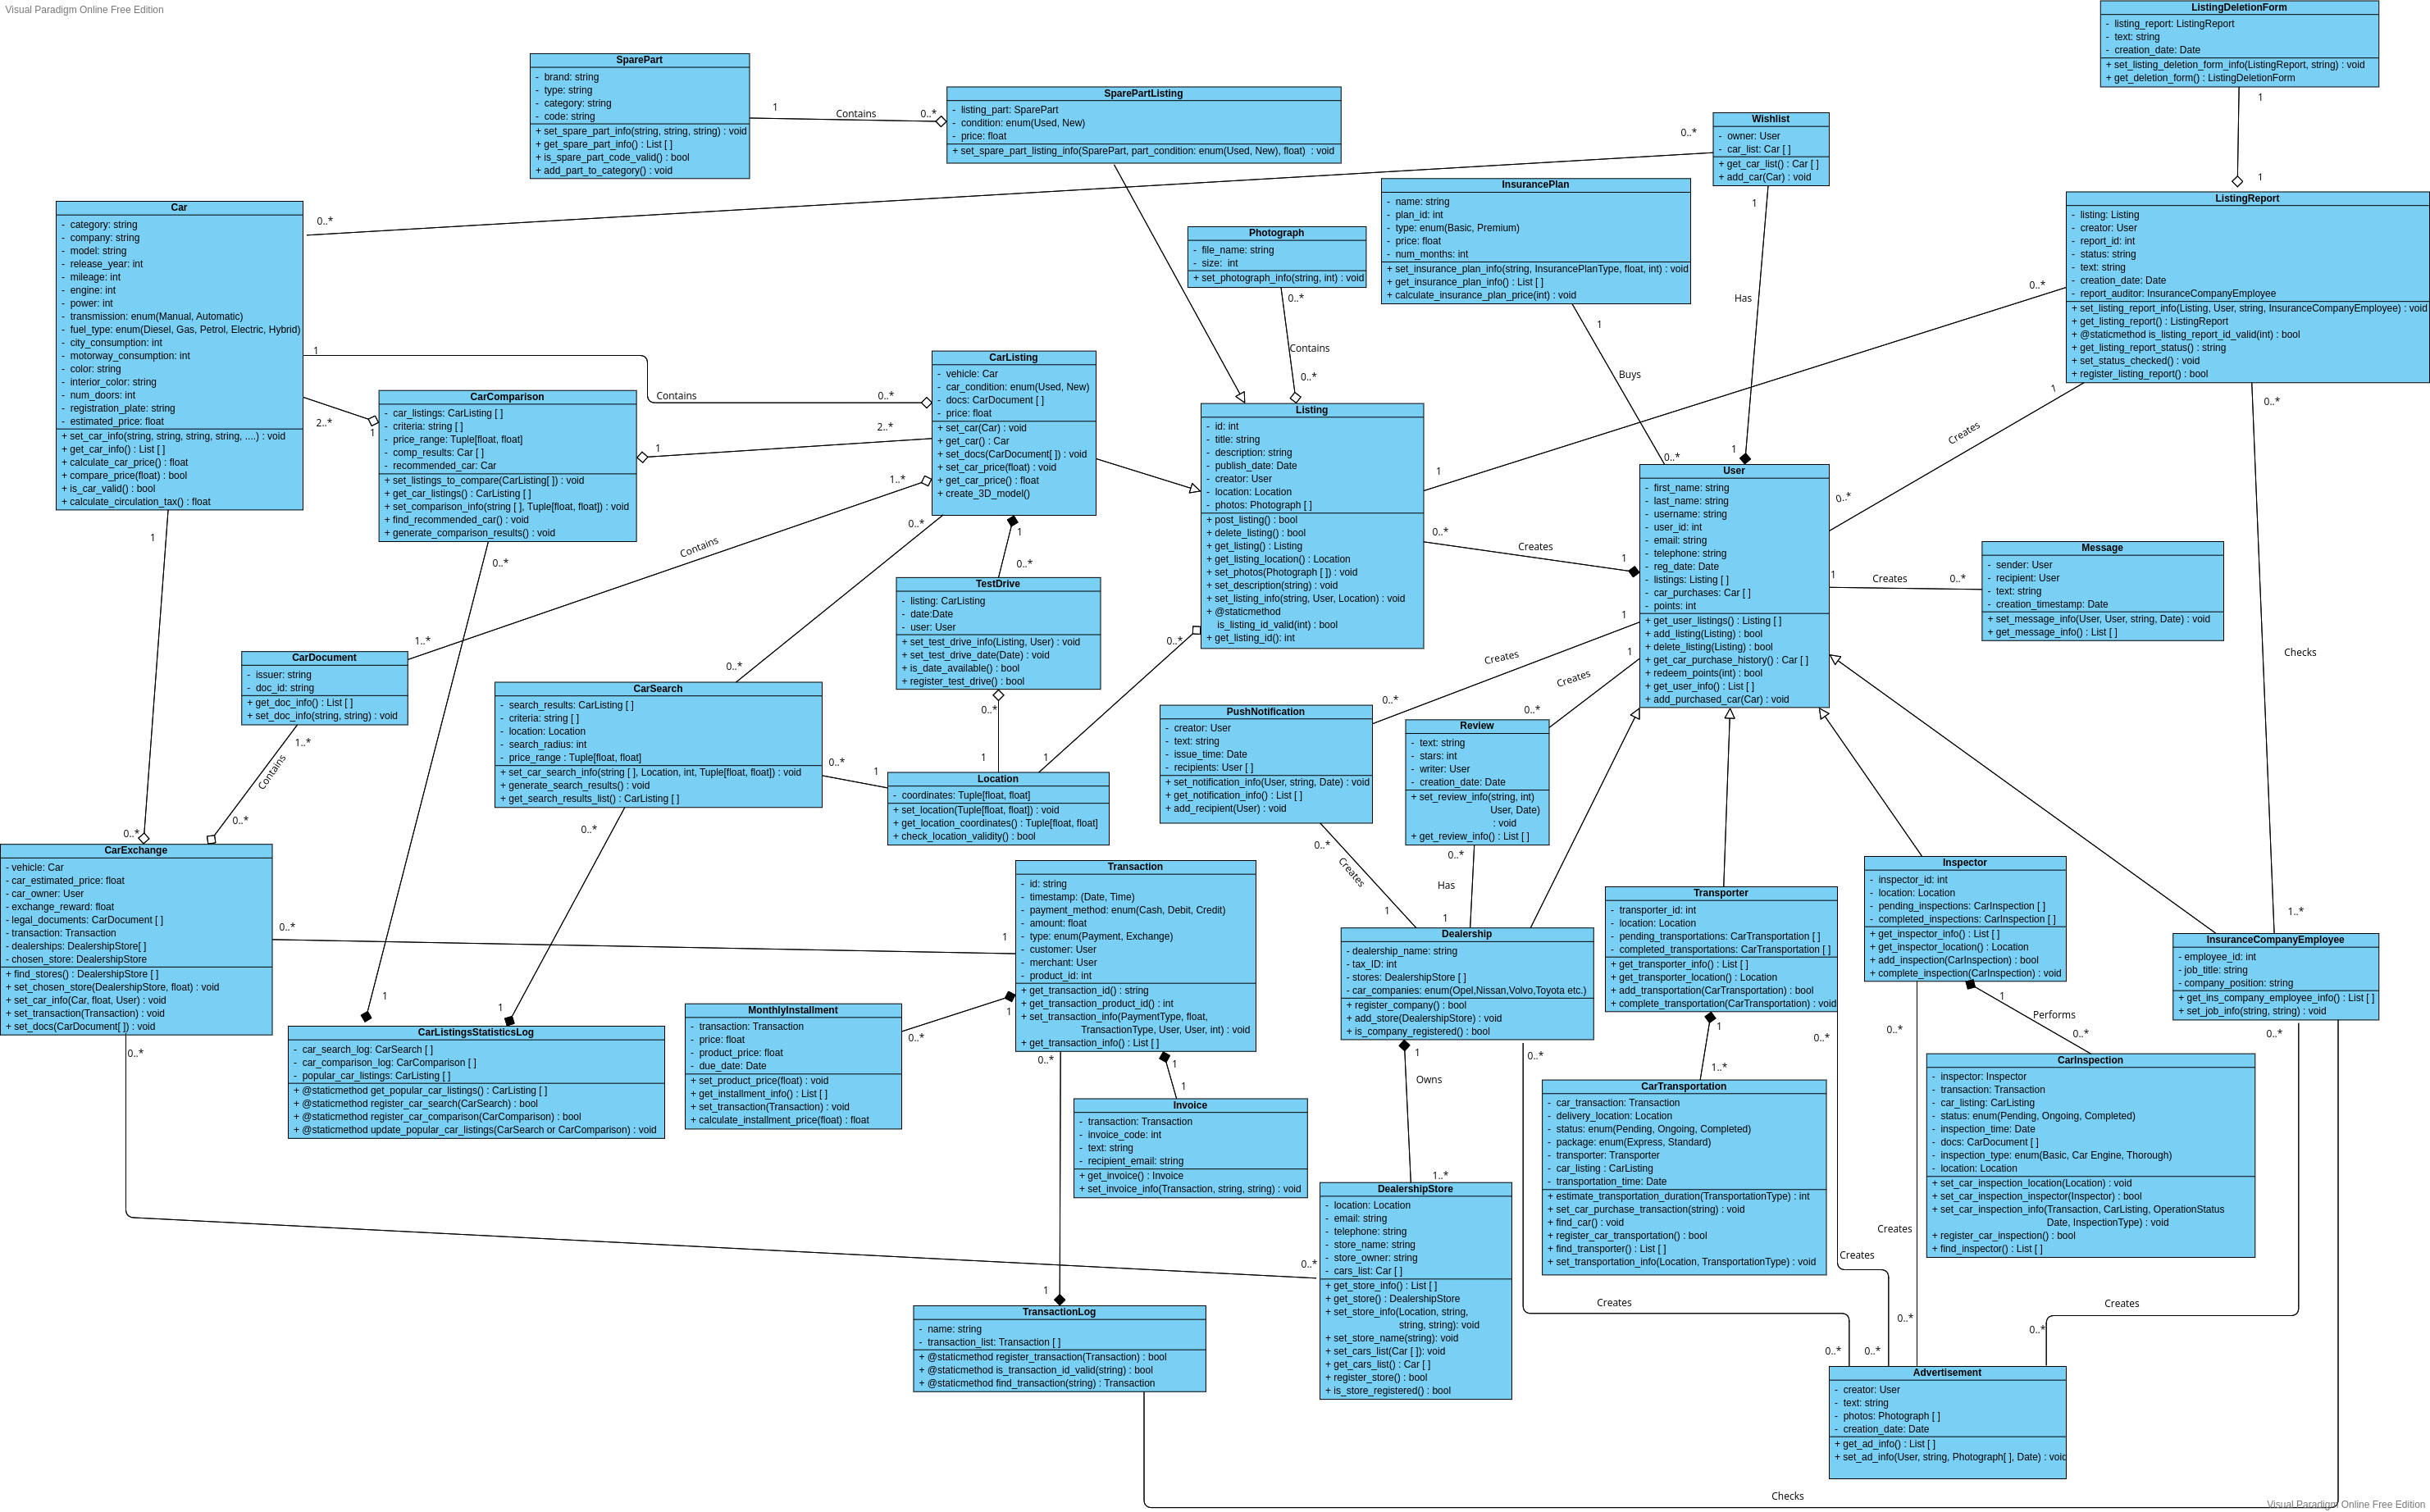
\includegraphics[width=\textwidth+3.4cm, height=15cm]{img/class_diagram_v0.2.png}
		\caption{\en UML Class Diagram \gr του \en Project \gr}
	\end{figure}
	
	
	
	\newpage
	
	\center{\textbf{Περιγραφή Κλάσεων}}
	
	\begin{itemize}
		\item \en \textbf{Car} \gr : Οντότητα που αντιστοιχεί σε ένα αυτοκίνητο και περιέχει όλα τα χαρακτηριστικά του (έτος κυκλοφορίας, μοντέλο κλπ)		
		\item \en \textbf{SparePart} \gr : Οντότητα που αντιστοιχεί σε ένα ανταλλακτικό και περιέχει όλα τα χαρακτηριστικά του
		\item \en \textbf{User} \gr : Γενική Οντότητα που αντιστοιχεί στον εγγεγραμμένο χρήστη της πλατφόρμας. Περιέχει χαρακτηριστικά του χρήστη, όπως το ονοματεπώνυμο, το \en username \gr, τον κωδικό του, το \en email \gr του, το τηλέφωνό του και την ημερομηνία εγγραφής του
		\item \en \textbf{Inspector} \gr : Ειδικότερη περίπτωση εγγεγραμμένου χρήστη, που αντιστοιχεί στους Ελεγκτές που διεξάγουν τους ελέγχους των οχημάτων. Περιέχει τον κωδικό του Ελεγκτή, την τοποθεσία του, καθώς και μια την λίστα με τους εκκρεμείς αλλά και ολοκληρωμένους ελέγχους οχημάτων του συγκεκριμένου Ελεγκτή
		\item \en \textbf{Transporter} \gr : Ειδικότερη περίπτωση εγγεγραμμένου χρήστη, που αφορά τους Μεταφορείς, ευθύνη των οποίων είναι η μεταφορά οχημάτων. Περιέχει τον κωδικό του Μεταφορέα, την μόνιμη τοποθεσία του Μεταφορέα, καθώς και μια την λίστα με τις εκκρεμείς αλλά και ολοκληρωμένες μεταφορές οχημάτων του συγκεκριμένου Μεταφορέα
		\item \en \textbf{Dealership} \gr : Ειδικότερη περίπτωση εγγεγραμμένου χρήστη, που αντιστοιχεί σε μια Αντιπροσωπεία Οχημάτων. Περιέχει πληροφορίες όπως το όνομα της εταιρείας, τον Αριθμό Φορολογικού Μητρώου της, μια λίστα με τα Καταστήματά της καθώς και μια λίστα με τις εταιρείες των οχημάτων που διαθέτει προς πώληση
		\item \en \textbf{InsuranceCompanyEmployee} \gr : Ειδικότερη περίπτωση εγγεγραμμένου χρήστη, που αντιστοιχεί σε υπάλληλο της Ασφαλιστικής Εταιρείας που διαχειρίζεται την πλατφόρμα. Περιέχει στοιχεία όπως, τον κωδικό του υπαλλήλου, το τμήμα της Ασφαλιστικής Εταιρείας στο οποίο εργάζεται, καθώς και τον τίτλο της θέσης του
		\item \en \textbf{Listing} \gr : Οντότητα που αντιστοιχεί σε μια αναρτημένη, στο σύστημα, αγγελία. Μπορεί να είναι είτε αγγελία πώλησης οχήματος (από Ιδιώτη ή από Αντιπροσωπεία), είτε αγγελία πώλησης ανταλλακτικού, είτε αγγελία που έχει αναρτήσει κάποιος Ελεγκτής προκειμένου να πληροφορήσει του χρήστες για τις υπηρεσίες που παρέχει. Περιέχει, μεταξύ άλλων, πληροφορίες όπως τον τίτλο της αγγελίας, τον κωδικό της και την περιγραφή της
		\item \en \textbf{CarListing} \gr : Ειδικότερη περίπτωση αναρτημένης αγγελίας, που αφορά αγγελία πώλησης οχήματος. Περιέχει το όχημα, την κατάστασή του, τα έγγραφά του και την τιμή του
		\item \en \textbf{SparePartListing} \gr : Ειδικότερη περίπτωση αναρτημένης αγγελίας, που αντιστοιχεί σε αγγελία πώλησης ανταλλακτικού. Περιέχει το ανταλλακτικό, την κατάστασή του, καθώς και την τιμή πώλησής του
		\item \en \textbf{ListingReport} \gr : Οντότητα που αντιστοιχεί σε Αναφορά αγγελίας. Περιέχει πληροφορίες όπως την υπό αναφορά αγγελία, τον χρήστη που δημιούργησε την αναφορά, τον κωδικό της αναφοράς, την κατάστασή της, το κείμενο με την αιτία υποβολής της αναφοράς, την ημερομηνία δημιουργίας της και τον υπάλληλο της Ασφαλιστικής Εταιρείας που εξέτασε την αναφορά
		\item \en \textbf{ListingDeletionForm} \gr : Οντότητα που αντιστοιχεί στην φόρμα διαγραφής αγγελίας, την οποία συμπληρώνει ο υπάλληλος της ασφαλιστικής εταιρείας, που εξετάζει την αναφορά που έχει δεχθεί μια αγγελία. Περιέχει πληροφορίες όπως το κείμενο με την αιτία διαγραφής της αγγελίας, την ημερομηνία δημιουργίας της φόρμας καθώς και τις πληροφορίες της αναφοράς της αγγελίας			
		\item \en \textbf{Transaction} \gr : Οντότητα που αντιστοιχεί σε μια συναλλαγή που διεξήχθη μέσω της πλατφόρμας και περιέχει όλα τα χαρακτηριστικά της, όπως κωδικός συναλλαγής, ποσό, ημερομηνία, τρόπος πληρωμής, τύπος Συναλλαγής, χρήστης πελάτης, χρήστης πωλητής και κωδικός προϊόντος
		\item \en \textbf{TransactionLog} \gr : Οντότητα που αντιστοιχεί στο μοναδικό και καθολικό Αρχείο Καταγραφής συναλλαγών (\en Log\gr), στο οποίο έχει πρόσβαση μόνο η Ασφαλιστική Εταιρεία. Έχει τίτλο και μια λίστα από τις συναλλαγές που έχουν διεξαχθεί
		\item \en \textbf{Message} \gr : Οντότητα που αντιστοιχεί σε μήνυμα που αποστέλλουν μεταξύ τους οι χρήστες της εφαρμογής και περιέχει χαρακτηριστικά όπως το \en username \gr του αποστολέα και του παραλήπτη, το κείμενο του μηνύματος και την ημερομηνία και ώρα δημιουργίας του μηνύματος
		\item \en \textbf{Location} \gr : Οντότητα που περιγράφει μια φυσική τοποθεσία με βάση το γεωγραφικό της στίγμα
		\item \en \textbf{Advertisement} \gr : Οντότητα που αντιστοιχεί σε μια διαφήμιση που έχει δημιουργηθεί είτε από μια Αντιπροσωπεία, είτε από έναν Μεταφορέα, είτε από έναν Ελεγκτή, είτε από την Ασφαλιστική Εταιρεία. Περιέχει το \en username \gr του δημιουργού της, το κείμενό της, μια λίστα από φωτογραφίες καθώς και την ημερομηνία δημιουργίας της
		\item \en \textbf{PushNotification} \gr : Οντότητα που αφορά τα \en Push Notifications \gr που μπορεί να δημιουργήσει μια Αντιπροσωπεία, είτε ειδοποιήσεις που εμφανίζονται στον χρήστη, πχ ως υπενθύμιση για ένα ραντεβού για \en Test Drive \gr. Περιέχει το \en username \gr του δημιουργού της ειδοποίησης, το κείμενό της, την ημερομηνία δημιουργίας, καθώς και μια λίστα με τα \en usernames \gr των παραληπτών
		\item \en \textbf{CarDocument} \gr : Οντότητα που αντιστοιχεί σε έγγραφα ενός οχήματος (είτε νομικά είτε πιστοποίησης κατάστασης). Περιέχει το όνομα του φορέα έκδοσης και έναν μοναδικό κωδικό
		\item \en \textbf{CarExchange} \gr : Οντότητα που αφορά μια Ανταλλαγή Οχημάτων που διεξάγεται μεταξύ ενός Ιδιώτη χρήστη και μιας Αντιπροσωπείας. Περιέχει, τα στοιχεία του οχήματος, την εκτιμώμενη τιμή του,  τα στοιχεία του χρήστη, την ανταμοιβή του, τα απαραίτητα έγγραφα, την αντίστοιχη Συναλλαγή, μια λίστα από τα καταστήματα Αντιπροσωπειών που δέχονται το όχημα και το κατάστημα που επιλέχθηκε από τον χρήστη
		\item \en \textbf{CarComparison} \gr : Οντότητα που αντιστοιχεί σε μια σύγκριση μεταξύ οχημάτων, και περιέχει στοιχεία όπως μια λίστα με τις αγγελίες των οχημάτων που συμμετέχουν στην σύγκριση, τα κριτήρια με βάση τα οποία γίνεται η σύγκριση, το εύρος τιμών, μια λίστα με τα αποτελέσματα της σύγκρισης καθώς και το προτεινόμενο από το σύστημα, όχημα
		\item \en \textbf{CarSearch} \gr : Οντότητα που αντιστοιχεί σε αναζήτησης οχήματος και περιέχει στοιχεία όπως την τοποθεσία του χρήστη, την ακτίνα αναζήτησης, μια λίστα με τις αγγελίες που συνιστούν τα αποτελέσματα της αναζήτησης, τα κριτήρια της αναζήτησης και το εύρος τιμών		
		\item \en \textbf{CarListingsStatisticsLog} \gr : Οντότητα που αντιστοιχεί στο μοναδικό και καθολικό Αρχείο Καταγραφής Αναζητήσεων και Συγκρίσεων Οχημάτων. Έχει μια λίστα από τις αναζητήσεις και συγκρίσεις οχημάτων που έχουν διεξαχθεί από τους χρήστες της πλατφόρμας, καθώς και μια λίστα με τις δημοφιλείς αγγελίες οχημάτων. Η κλάση αυτή χρησιμοποιείται προκειμένου, να μπορεί να διεξαχθεί στατιστική ανάλυση στις αναζητήσεις των χρηστών, και να εξαχθούν οι δημοφιλείς αγγελίες που εμφανίζονται συχνά στις αναζητήσεις και τις συγκρίσεις		
		\item \en \textbf{CarInspection} \gr : Οντότητα που αφορά προγραμματισμένο έλεγχο οχήματος και περιέχει, στοιχεία όπως, τον Ελεγκτή που θα πραγματοποιήσει τον έλεγχο, την Συναλλαγή πληρωμής του Ελέγχου, την αγγελία του υπό εξέταση οχήματος, την κατάστασή του (εκκρεμής/σε εξέλιξη/ολοκληρωμένος), την ημερομηνία και ώρα διεξαγωγής του, τα έγγραφα πιστοποίησης κατάστασης που θα προκύψουν, τον τύπο του ελέγχου αλλά και την τοποθεσία διεξαγωγής του
		\item \en \textbf{CarTransportation} \gr : Οντότητα που αντιστοιχεί σε μια προγραμματισμένη μεταφορά οχήματος, και περιέχει στοιχεία όπως, την Συναλλαγή αγοράς του οχήματος, την τοποθεσία παράδοσης του οχήματος, την κατάστασή του (εκκρεμής/σε εξέλιξη/ολοκληρωμένος), τον τύπο της μεταφοράς (Κανονική ή \en Express\gr), τον Μεταφορέα, την αγγελία του οχήματος και την ημερομηνία 
		\item \en \textbf{TestDrive} \gr : Οντότητα που αντιστοιχεί σε ένα προγραμματισμένο ραντεβού για \en Test Drive \gr ενός οχήματος. Περιέχει πληροφορίες όπως την αγγελία του οχήματος, την ημερομηνία του ραντεβού καθώς και τα στοιχεία του χρήστη που προγραμμάτισε το ραντεβού
		\item \en \textbf{InsurancePlan} \gr : Οντότητα που αφορά ένα Ασφαλιστικό Πακέτο και περιέχει χαρακτηριστικά όπως τον κωδικό του πακέτου, το όνομα του πακέτου, τον τύπο του, τα μηνιαία ασφάλιστρα και την διάρκεια του πακέτου σε μήνες
		\item \en \textbf{MonthlyInstallment} \gr : Οντότητα που αφορά την Μηνιαία Δόση εξόφλησης της αγοράς ενός οχήματος και περιέχει στοιχεία όπως τα στοιχεία της συναλλαγής αγοράς του οχήματος, το ποσό της δόσης, την τιμή του προϊόντος που εξοφλείται και την καταληκτική ημερομηνία καταβολής της δόσης
		\item \en \textbf{Invoice} \gr : Οντότητα που αφορά την Απόδειξη Συναλλαγής. Περιέχει τις πληροφορίες της Συναλλαγής, τον κωδικό της απόδειξης, το κείμενό της και το \en email \gr του παραλήπτη της	
		\item \en \textbf{Review} \gr : Οντότητα που αντιστοιχεί σε κριτική που μπορεί να έχει δεχθεί ένα Ιδιώτης ή μια Αντιπροσωπεία. Περιέχει χαρακτηριστικά όπως το κείμενο της κριτικής, τον αριθμό των αστεριών, το \en username \gr του δημιουργού, την ημερομηνία της δημιουργίας
		\item \en \textbf{Wishlist} \gr : Οντότητα που αντιστοιχεί στην \en Wishlist \gr ενός χρήστη. Περιέχει τα στοιχεία του κατόχου της και μια λίστα από οχήματα
		\item \en \textbf{DealershipStore} \gr : Οντότητα που αντιστοιχεί σε Φυσικό Κατάστημα που υπάγεται σε μια Αντιπροσωπεία Οχημάτων. Περιλαμβάνει στοιχεία όπως, την τοποθεσία του, το \en email\gr και το τηλέφωνο επικοινωνίας, το όνομα του καταστήματος, το όνομα του ιδιοκτήτη του καταστήματος αλλά και μια λίστα με τα οχήματα που διαθέτει προς πώληση
	\end{itemize}
	
	
	
	
	
\end{document}
